\documentclass[english]{article}
\usepackage[utf8]{inputenc}
\usepackage[T1]{fontenc}
\usepackage{babel}
\usepackage{amsmath}
\usepackage{graphicx}
\usepackage{fancyhdr}
\usepackage{lscape}
\newcommand{\scidatalogo}{
\includegraphics[height=36pt]{img/SciData_logo.jpg}}
\pagestyle{fancy}
\fancyhf{}
\renewcommand{\headrulewidth}{0pt}
\setlength{\headheight}{40pt}
\lhead{\textsc{\scidatalogo}}

% command for column names and table names
 \newcommand{\colname}[1]{\texttt{#1}}
 \newcommand{\tblname}[1]{\emph{#1}}

% pretty symbols for the table (checkmark / cross-mark)
\usepackage{pifont}
\newcommand{\cmark}{\ding{51}}%checkmark
\newcommand{\xmark}{\ding{55}}%x

\begin{document}

\title{The eICU Collaborative Research Database, a freely available multi-center database for critical care research}

\author{Tom J. Pollard\textsuperscript{1{$\dagger$}}
\and Alistair E. W. Johnson\textsuperscript{1{*}{$\dagger$}}
\and Jesse D. Raffa\textsuperscript{1}
\and Leo A. Celi\textsuperscript{1,2}
\and Roger G. Mark\textsuperscript{1,2}
\and Omar Badawi\textsuperscript{1,3,4}}

\maketitle
\thispagestyle{fancy}

1. Institute for Medical Engineering and Science, Massachusetts Institute of Technology, Cambridge, MA, USA.

2. Beth Israel Deaconess Medical Center, Boston, MA, USA.

3. Department of eICU Research and Development, Philips Healthcare, Baltimore, MD, USA.

4. Department of Pharmacy Practice and Science, University of Maryland, School of Pharmacy, Baltimore, MD, USA.

{$\dagger$} Contributed equally to this work.


{*}corresponding author:
Alistair E. W. Johnson (aewj@mit.edu)
\begin{abstract}
Critical care patients are monitored closely through the course of their illness. As a result of this monitoring, large amounts of data are routinely collected for these patients.
Philips Healthcare has developed a telehealth system, the eICU Program, which leverages these data to support management of critically ill patients.
Here we describe the eICU Collaborative Research Database, a multi-center intensive care unit (ICU) database with high granularity data for over 200,000 admissions to ICUs monitored by eICU Programs across the United States.
The database is deidentified, and includes vital sign measurements, care plan documentation, severity of illness measures, diagnosis information, treatment information, and more.
Data are publicly available after registration, including completion of a training course in research with human subjects and signing of a data use agreement mandating responsible handling of the data and adhering to the principle of collaborative research.
The freely available nature of the data will support a number of applications including the development of machine learning algorithms, decision support tools, and clinical research.
\end{abstract}

\section*{Background \& Summary}

% --- REQUIREMENTS OF THIS SECTION --- %
% (700 words maximum) An overview of the study design, the assay(s)
% performed, and the created data, including any background information
% needed to put this study in the context of previous work and the literature.
% The section should also briefly outline the broader goals that motivated
% the creation of this dataset and the potential reuse value. We also
% encourage authors to include a figure that provides a schematic overview
% of the study and assay(s) design. This section and the other main
% body sections of the manuscript should include citations to the literature
% as needed~\cite{cite1, cite2}. References should be included within the
% manuscript file itself as our system cannot accept BibTeX bibliography files.
% Authors who wish to use BibTeX to prepare their references should therefore
% copy the reference list from the .bbl file that BibTeX generates and paste it
% into the main manuscript .tex file (and delete the associated
% \textbackslash{}bibliography and \textbackslash{}bibliographystyle commands).
% ------------------------------------ %


Intensive care units (ICUs) provide care for severely-ill patients who require invasive life-saving treatment. Critical care as a subspecialty of medicine began during a polio epidemic in which large number of patients required mechanical ventilation for many weeks~\cite{kelly2014intensive}. Since then, the field of critical care has grown, and continues to evolve as demographics shift toward older and chronically sicker populations~\cite{adhikari2010critical}.
Patients in ICUs are monitored closely to detect physiologic changes associated with deteriorating illness and consequently reassess the treatment regimen as appropriate.
Close observation of ICU patients is facilitated by bedside monitors which continuously stream huge quantities of data, and relatively small portions of these data are archived for clinical documentation~\cite{Celi2013loop}.
Challenges of archiving these data include integration of disparate information systems and building a comprehensive system to handle all types of data~\cite{johnson2016machine}.

A telehealth ICU, or teleICU, is a centralized model of care where remote providers monitor ICU patients continuously, providing both structured consultations and reactive alerts~\cite{lilly2014multicenter}. TeleICUs allow caregivers from remote locations to monitor treatments for patients, alert local providers to sudden deterioration, and supplement care plans.
Philips Healthcare, a major vendor of ICU equipment and services, provide a teleICU service known as the eICU program.
Care providers primarily access and document data in an information management system called eCareManager and additionally have access to the other information systems present in the hospital.
After implementation of the eICU program, large amounts of data are collected and streamed for real-time monitoring by a remote ICU team.
These data are archived by Philips and transformed into a research database by the eICU Research Institute (eRI)~\cite{mcshea2010eicu}.


% Motivate sharing large dataset
The Laboratory for Computational Physiology (LCP) partnered with the eRI to produce the eICU Collaborative Research Database (eICU-CRD), a publicly available database sourced from the eICU Telehealth Program (Data Citation 1).
The LCP has previously shared the Medical Information Mart for Intensive Care (MIMIC) database~\cite{MIMIC2011, MIMIC2016}. The latest version, MIMIC-III, contains rich deidentified data for over 60,000 ICU admissions to the Beth Israel Deaconess Medical Center in Boston, MA. MIMIC-III has been used for education purposes, to investigate novel clinical relationships, and develop new algorithms for patient monitoring. The source hospital of MIMIC-III does not participate in the eICU programme, so eICU-CRD is a completely independent set of data collected from a large number of hospitals located within the United States. The release of eICU-CRD is intended to build upon the success of MIMIC-III and expand the scope of studies possible by making data available from multiple centers.

\section*{Methods}

% --- REQUIREMENTS OF THIS SECTION --- %
% The Methods should include detailed text describing any steps or procedures
% used in producing the data, including full descriptions of the experimental
% design, data acquisition assays, and any computational processing (e.g.
% normalization, image feature extraction). Related methods should be grouped
% under corresponding subheadings where possible, and methods should be described
% in enough detail to allow other researchers to interpret and repeat, if required,
% the full study. Specific data outputs should be explicitly referenced via data
% citation (see Data Records and Data Citations, below). Authors should

% previous descriptions of the methods under use, but ideally the method
% descriptions should be complete enough for others to understand and reproduce
% the methods and processing steps without referring to associated publications.
% There is no limit to the length of the Methods section.
% ------------------------------------ %


\subsection*{Database structure and development}\label{database-structure-and-development}

The eICU Collaborative Research Database is distributed as a set of comma separated value (CSV) files which can be loaded into any relational database system. Each file contains data for a single table, and we denote references to tables by using \tblname{italicized font}. Similarly, we denote references to columns using \colname{monospace font}.

All tables are deidentified to meet the safe harbor provision of the US Health Insurance Portability and Accountability Act (HIPAA)~\cite{HIPAA}. These provisions include the removal of all protected health information (PHI), such as personal numbers (e.g. phone, social security), addresses, dates, and ages over 89. When creating the dataset, patients were randomly assigned a unique identifier and a lookup key was not retained. As a result the identifiers in eICU-CRD cannot be linked back to the original, identifiable data. All hospital and ICU identifiers have also been removed to protect the privacy of contributing institutions and providers.

The schema was established in collaboration with Privacert (Cambridge, MA), who certified the re-identification risk as meeting safe harbor standards (HIPAA Certification no. 1031219-2). Subsequent to this certification, free-text fields were scanned for personal information using a previously published rule-based approach~\cite{neamatullah2008automated}. Briefly, this approach scans text for known patterns indicating presence of PHI (e.g. words following ``Mr.'' are frequently names, such as ``Mr. Smith''). The approach also detects words which are commonly used as places or names. The output of this algorithm was reviewed, and rows containing potential PHI were deleted. Finally, large portions of all tables were manually reviewed by at least three personnel to verify all data had been deidentified. Frequently, due to a low number of unique entries (e.g. when a table stored the results of a drop-down menu), the entire table was reviewed.

The schema of eICU-CRD is highly denormalized. All tables can be accessed independently and linked to a single patient tracking table, \tblname{patient}, using \colname{patientUnitStayId}. The only exception to this is the hospital table, which links to the patient table using \colname{hospitalId}. All tables, other than \tblname{patient} and \tblname{hospital}, have a randomly generated primary key with the suffix `id' (for example, the \tblname{diagnosis} table has \colname{diagnosisId} as a primary key). This column has no physical meaning, being used only to constrain uniqueness on rows and ensure integrity of the data when loading into a database system.

\subsection*{Patient identifiers}\label{patient-identifiers}

Unit stays, where the primary unit of care is the ICU, are identified by a single integer: the \colname{patientUnitStayId}. Each unique hospitalization is also assigned a unique integer, known as the \colname{patientHealthSystemStayId}. Finally, patients are identified by a \colname{uniquePid}. Unlike the other identifiers, \colname{uniquePid} is generated using an algorithm based upon prior work on linking disparate patient medical records~\cite{finney2011efficient}.
Each \colname{patientHealthSystemStayId} has at least one or more \colname{patientUnitStayId}, and each \colname{uniquePid} can have multiple hospital and/or unit stays. Figure \ref{fig:patient_organization} visualizes this hierarchy. All tables use
\colname{patientUnitStayId} to identify an individual unit stay, and the patient table can be used to determine unit stays linked to the same patient and/or hospitalization.

\begin{figure}[htbp]
\centering
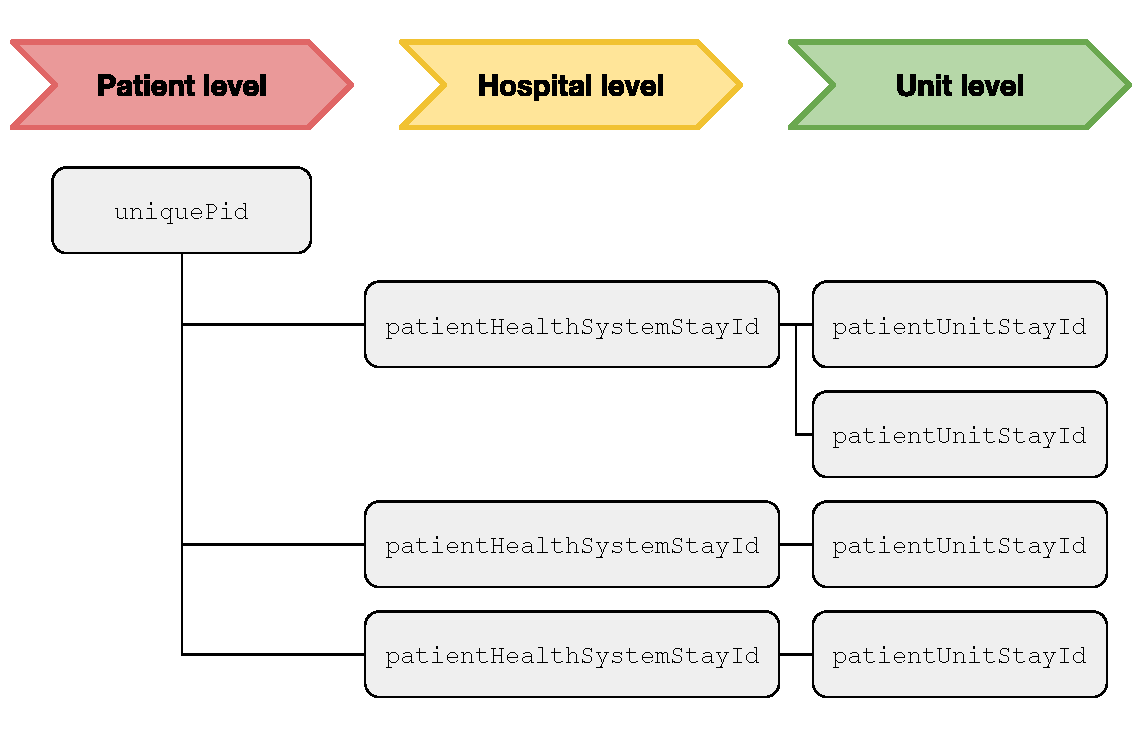
\includegraphics[width=0.70000\textwidth]{img/Patient_Organization}
\caption{\emph{Organization of patient tracking information.} Each patient is identified by a unique integer: the \colname{uniquePid}. For each \colname{uniquePid}, a patient may have distinct hospitalizations denoted by \colname{patientHealthSystemStayId}. Finally, for each hospitalization, a patient may have distinct unit stays, denoted by \colname{patientUnitStayId}. \colname{patientUnitStayId} is the primary identifier used for linking data across tables. \label{fig:patient_organization}}
\end{figure}


\subsection*{Sample selection}\label{sample-selection}

The eICU Collaborative Research Database is a subset of a research data repository maintained by eRI.
A stratified random sample of patients was used to select patients for
inclusion in the public dataset. The selection was done as follows: first, all
hospital discharges between 2014 and 2015 were identified, and a single
index stay for each unique patient was extracted. The proportion of
index stays in each hospital from the eRI data repository was used to
perform a stratified sample of patient index stays based upon hospital;
the aim was to maintain the distribution of first ICU stays across the
hospitals in the dataset. After a patient index stay was selected, all
subsequent stays for that patient were also included in the dataset,
regardless of the admitting hospital. A small proportion of patients
only had stays in step down units or low acuity units, and these stays
were removed.

\subsection*{Code availability}

% --- REQUIREMENTS OF THIS SECTION --- %
%For all studies using custom code in the generation or processing of datasets,
%a statement must be included here, indicating whether and how the code can be
%accessed, including any restrictions to access. This section should also include
%information on the versions of any software used, if relevant, and any specific
%variables or parameters used to generate, test, or process the current dataset.
% ------------------------------------ %

A Jupyter Notebook containing the code used to generate the tables and descriptive statistics included in this paper is available online~\cite{eicu-data-paper}.

The code that underpins the eICU-CRD website and documentation is openly available and contributions from the research community are encouraged~\cite{eicu-code}.

\section*{Data Records}\label{data-records}

The database comprises 200,859 patient unit encounters for 139,367 unique
patients admitted between 2014 and 2015. Patients were admitted to one
of 335 units at 208 hospitals located throughout the US. Table \ref{tab:demographics} provides demographics of the dataset, including hospital level characteristics~\cite{tableone}.

Table \ref{tab:apachedx} highlights the top 10 most frequent admission diagnoses in the dataset as coded by trained eICU clinicians using the APACHE IV
diagnosis system~\cite{zimmerman2006acute}.
Table \ref{tab:apachedx_groups} collapses APACHE
diagnoses into 21 groups which are more clinically intuitive. Patients
who are missing APACHE IV hospital mortality predictions are excluded
from both tables (N=64,623). Patients will not have an APACHE IV
hospital mortality prediction if they satisfy exclusion criteria for
APACHE IV (burns patients, in-hospital readmissions, some transplant
patients), or if their diagnosis is not documented within the first day
of their ICU stay.

\subsection*{Classes of data}\label{classes-of-data}

Data include vital signs, laboratory measurements, medications, APACHE
components, care plan information, admission diagnosis, patient history,
time-stamped diagnoses from a structured problem list, and similarly
chosen treatments. The data are organized into tables which broadly
correspond to the type of data contained within the table. Table \ref{tab:tables_available} gives
an overview of tables available in the dataset.

\subsubsection*{Administrative data}\label{administrative-data}

Hospital level information is available in the \tblname{hospital} table, and includes regional location in the USA (midwest, northeast, west, south), teaching status, and the number of hospital beds. Hospital information is the result of a survey and is sometimes incomplete: 12.5\% have unknown region and 20.1\% have unknown bed capacity. Table \ref{tab:hospital_info} shows the percentage of hospital data in each category.

Patient information is recorded in the \tblname{patient} table. The three identifiers described earlier (\colname{patientUnitStayId}, \colname{patientHealthSystemStayId}, \colname{uniquePid}) are present in this table. Administrative information recorded in the \tblname{patient} table includes: admission and discharge time, unit type, admission source, discharge location, and patient vital status on discharge. Patient demographics are also present in the \tblname{patient} table, including age (with ages \textgreater{} 89 grouped into `\textgreater{} 89'), ethnicity, height, and weight.

\subsubsection*{APACHE data}\label{apache-data}

The Acute Physiology, Age, and Chronic Health Evaluation (APACHE) IV system~\cite{zimmerman2006acute}
is a tool used to risk-adjust ICU patients
for ICU performance benchmarking and quality improvement analysis. The
APACHE IV system, among other predictions, provides estimates of the
probability that a patient dies given data from the first 24 hours.
These predictions, on aggregate across many patients, can be used to
benchmark hospitals and subsequently identify policies from hospitals
which may be beneficial for patient outcomes. In order to make these
predictions, care providers must collect a set of parameters regarding
the patient: physiologic measurements, comorbid burden, treatments
given, and admission diagnosis. These parameters are used in a logistic
regression to predict mortality. eICU-CRD contains all parameters used
in the APACHE IV equations: physiologic parameters are primarily stored
in \tblname{apacheApsVar}, and other parameters are stored in
\tblname{apachePredVar}. The result of the predictions for both the
APACHE IV and the updated APACHE IVa equation are available in
\tblname{apachePatientResult}. These data provide an informative estimate
of patient severity of illness on admission to the ICU, though it should
be noted that these predictions are not available for every patient, in
particular: those who stay less than 4 hours, burns patients, certain
transplant patients, and in-hospital readmissions. See the original
publication for more detail~\cite{zimmerman2006acute}.

\subsubsection*{Care plan}\label{care-plan}

The care plan is a section of eCareManager which is primarily used for
intraprofessional communication. The data are documented using structured
multiple choice lists and is used to communicate care provider type,
provider specialty, code status, prognosis, treatment status, goals of
care, healthcare proxies, and end-of-life discussion.

\subsubsection*{Care documentation}\label{care-documentation}

Drop down lists available in eCareManager allow for structured
documentation of active problems and active treatments for a patient.
It is also possible for care staff to enter short free-text entries.
Eighteen tables are available in eICU-CRD which document various aspects of each patient's care including measurements made, active problems, treatments planned, and more.

\tblname{admissionDrug}. This table contains details of medications that a patient was taking prior to admission to the ICU.
Information available includes the drug name, dosage, time frame during which the drug was administered, the user type and specialty of the clinician entering the data, and the note type where the information was entered.

\tblname{allergy}. Allergies were documented in the \tblname{allergy} table and sourced from patient note forms. Allergy information is available with a free text allergy name, type of documenting caregiver, whether the allergy is a drug, a standardized code for the drug (if applicable), and the time at which the allergy was documented.

\tblname{customLab}. Laboratory measurements that are not configured within the standard interface are included in the \tblname{customLab} table. These laboratory measurements are infrequently measured but may provide useful information for a small subset of patients. The most frequently measured test in the \tblname{customlab} table is glomerular filtration rate (GFR), and the table contains data for less than 1\% of all patients in eICU-CRD v2.0.

\tblname{diagnosis}. Active problems were documented in the \tblname{diagnosis} table,
with 86\% of patients having a documented active problem during
the first 24 hours of their unit stay. There were a total of 3,933
unique active problems; the most common was acute respiratory failure
(11.15\% of patients), followed by acute renal failure (8.15\% of
patients) and diabetes (7.28\% of patients). Problems are hierarchically
categorized, and Table \ref{tab:organ_system} shows the proportion of patients with an active problem for each organ system. Note that a patient can have problems
documented for multiple organ systems.
Most problems are mapped to International Classification of Disease (ICD) codes to facilitate identification of specific diseases using a well established ontology. However, it was not possible to map some diagnoses to ICD codes. For example, ``endocrine|glucose metabolism|diabetes mellitus|Type II|controlled'' is mapped to ICD-9 code 250.00 (Diabetes mellitus without mention of complication, type II or unspecified type, not stated as uncontrolled) and ICD-10 code E11.9 (Type 2 diabetes mellitus without complications).
However, ``endocrine|glucose metabolism|diabetes mellitus'' is not mapped to an ICD code, as it is not clear whether this is type I or type II.

\tblname{infusionDrug}. Details of drug infusions are recorded within the \tblname{infusionDrug} table. These infusions are entered by care staff manually or interfaced from an electronic health record system from the hospital. Continuous infusions documented include vasopressors, antibiotics, anticoagulation, insulin, sedatives, analgesics, and so on. Of the 208 hospitals in eICU-CRD, 152 (73\%) have data recorded in the \tblname{infusionDrug} table. Recorded information includes the name of the drug, a standardized code for the drug (using Hierarchical Ingredient Code List or HICL codes), the amount of drug in the carrying solution, the total volume of the carrier, the rate of the drug infusion, and the patient weight (if applicable for dosing). All records are stored with a single offset representing the time of the infusion.

\tblname{intakeOutput}. The intake and output of any volume for patients is stored in the \tblname{intakeOutput} table. Unlike the \tblname{infusionDrug} table, the aim of this table is to tabulate volume received, and thus many records exist with non-specific names such as ``Crystalloids (ml)|Continuous infusion meds''.
Overall fluid balance is an important aspect of patient health, and running totals for intake, output, dialysis, and net (intake minus output) are recorded. The most frequent records in the \tblname{intakeOutput} table include urine output, infusion of normal saline, oral fluid intake, non-saline fluid administration (e.g. dextrose based), enteral feeding, parenteral feeding, and more.

\tblname{lab}. Laboratory values collected during routine care are interfaced with
eCareManager and archived in the database.
Each row of the \tblname{lab} table contains a single laboratory measurement for a patient.
Each hospital has had their local laboratory measurements mapped to standard concepts.
A total of 158 distinct types of laboratory measurements are captured and represented by 158 unique \colname{labName} values (including ``magnesium'', ``pH'', ``BUN'', etc).
Measurements are stored with the unit of measurement, the time the lab was drawn,
and the last time the value was revised.

\tblname{medication}. Active medication orders for patients are stored in the \tblname{medication} table.
When a medication order is made by a physician, a pharmacist will review and verify the order in their corresponding pharmacy system. This order verification is interfaced into eCareManager and stored in the \tblname{medication} table. Free text instructions and comments are removed during the deidentification process.
In eICU-CRD, two tables focus on recording patient medication: \tblname{medication} and \tblname{infusionDrug}.
There are two key differences between these tables: (1) only continuous infusions are present in \tblname{infusionDrug} (e.g. intravenously infused normal saline but not orally prescribed acetaminophen), and (2) compounds described in \tblname{medication} are orders; and while usually these orders are fulfilled and administered this cannot be guaranteed. Information available for each order includes: the start time, end time, name of the compound, HICL code, dosage, route of administration, frequency of administration, loading dose, whether the drug is given pro re nata (PRN), and whether the drug is an IV admixture.

\tblname{microLab}. Microbiology information from patient derived specimens is made available in the \tblname{microLab} table. Presence of bacteria in specimens such as blood or sputum provides useful information for treatment planning and selection of antibiotic regimen. For each record the time of specimen collection (e.g. blood draw), site of the culture, organism found (if any), and sensitivity to various antibiotics (if any are tested).
As microbiology is documented manually by care providers, and not directly interfaced from local hospital information systems, the table is not populated for a significant number of hospitals.

\tblname{note}. Notes are generally entered by the physician or physician extender primarily responsible for the documentation of the patient's unit care. There are several types of notes which can be entered in the system including admission, progress, patient medical history, procedure, catheterization, and consultation. Free-text notes were removed during the deidentification process. Highly structured text notes which are selected from drop down menus are retained within the database and present in the \tblname{note} table.

\tblname{nurseAssessment}. The nursing assessment table stores information about the capability to assess and document patient items such as pain, psychosocial status, patient/family education, and organ specific statuses. Each record in the table is stored with the time of documentation and the time at which the assessment is relevant.

\tblname{nurseCare}. Patient care information is documented in the \tblname{nurseCare} table for the following categories: nutrition, activity, hygiene, wound care, line care, drain status, patient safety, alarms, isolation precautions, equipment, restraints, and other nursing care data.
Each record is stored with an entry time (\colname{nurseCareEntryOffset}) and a relevant time (\colname{nurseCareOffset}). A custom hierarchy is used to group and store data.

\tblname{nurseCharting}. The majority of bedside documentation is entered into a ``flowsheet'', a tabular style interface with time in columns (usually hourly) and observations in rows. The \tblname{nurseCharting} table contains this information using a entity-attribute-value model, where the entity is a patient identifier, the attribute is the type of data recorded (e.g. heart rate), and the value is the measurement made (e.g. 80 beats per minute).
Each charted item is stored with a ``chart time'' (\colname{nursingChartOffset}), which specifies when the measurement was relevant, and a ``validation time'' (\colname{nursingChartEntryOffset}), which indicates when the measurement was verified by staff.
Vital signs available include: heart rate, heart rhythm, blood pressure, respiratory rate, peripheral oxygen saturation, temperature, location of temperature measurement, central venous pressure, oxygen flow in liters,  oxygen device used for oxygen flow, and end tidal CO2.
Less frequently documented vital signs available include: pulmonary artery pressure (PA), stroke volume (SV), cardiac output (CO), systemic vascular resistance (SVR), intracranial pressure (IP), cardiac index (CI), systemic vascular resistance index (SVRI), cerebral perfusion pressure (CPP), central venous oxygen saturation (SVO2),  pulmonary artery occlusion pressure (PAOP), pulmonary vascular resistance (PVR), pulmonary vascular resistance index (PVRI), and intra-abdominal pressure (IAP).
Other data elements available in \tblname{nurseCharting} include assessments made, commonly tabulated scores (neurological function scales, sedation scales, pain scales), and other physiologic measurements or device settings.

\tblname{pastHistory}. Information related a patient's relevant past medical history is stored in the \tblname{pastHistory} table.
Providing a detailed past history is not common, but items such as AIDS, cirrhosis of the liver, hepatic failure, chronic renal failure, transplant, pre-existing cancers, and immunosuppression are more reliably documented due to their importance in severity of illness scoring. Elements of past medical history are documented using a custom hierarchical coding system and stored with the charted time (\colname{pastHistoryOffset}) and with the entry time (\colname{pastHistoryEntryOffset}).

\tblname{physicalExam}. Results of physical exams performed are stored in the \tblname{physicalExam} table. Data for physical exams are entered directly into eCareManager. The choices for the physical exam include "Not Performed", "Performed-Free Text", and "Performed-Structured". Free text sections are not included in the database. There is a large variety of drop-down menus for the physical exams recorded, with specific text entry boxes allowing for the creation of a structured physical exam.

\tblname{respiratoryCare}. This table contains information related to respiratory care. Patient data include respiratory care times, sequence of records for historical ordering, airway type/size/position, cuff pressure and various other ventilation details. Unlike other tables, the \tblname{respiratoryCare} table does not use an entity-value-attribute model, but instead has many columns for each setting, most of which are empty for a given time of data recording.

\tblname{respiratoryCharting}. Charted data which relate to a patient's ventilation status, including the configuration of the bedside mechanical ventilator, are stored in the \tblname{respiratoryCharting} table.
Each setting is stored with an entry time (\colname{respChartEntryOffset}) and an observation time (\colname{respChartOffset}).
Examples of settings include the percentage of oxygen inspired, tidal volumes, pressure settings, and other ventilator parameters.

\tblname{treatment}: A custom hierarchical coding system is used to record
active treatments, and there are are 2,711 unique treatments documented
in eICU-CRD. The most frequent treatments explicitly documented in the table
across patients were mechanical ventilation (16.96\% of patients), chest
x-rays (8.79\% of patients), oxygen therapy via a nasal cannula with a
low fraction of oxygen (6.93\% of patients), and normal saline
administration (7.57\%).

\subsubsection*{Bedside monitor data}\label{monitor-data}

Large quantities of data are continuously recorded on ICU patients and
displayed via bedside monitors. The \tblname{vitalPeriodic} and
\tblname{vitalAperiodic} tables contain data derived directly from these
bedside monitors.
Unlike other data elements in the database, the data collected in these tables are not entered or validated by providers of care: the periodic and aperiodic vital sign data have been automatically derived and archived with no human verification.

\tblname{vitalPeriodic}. Continuously measured vital signs are recorded in the \tblname{vitalPeriodic} table
and include heart rate, respiratory rate,
oxygen saturation, temperature, invasive arterial blood pressure,
pulmonary artery pressure, ST levels, and intracranial pressure (ICP).
Vital signs are originally collected at 1-minute intervals, with 5-minute medians archived in eICU-CRD.
Table \ref{tab:vitalperiodic} summarizes data completion for periodic vital signs.
The most frequently available periodic vital sign is heart rate
(available for 96\% of patients), and the least available periodic vital
sign is ICP (available for 0.81\% of patients).
Conversely, while the average number of heart rate measurements among
patients with at least one recording of heart rate is 759.2 (approximately 63 hours),
the average number of ICP measurements among patients with at least one ICP measurement is much higher
at 1610.3 (approximately 134 hours). Thus, while monitoring of ICP is infrequent across all patients,
when it is performed it results in a large number of recordings.


\tblname{vitalAperiodic}. Aperiodic vital signs are collected at various times and include
non-invasive blood pressure, pulmonary artery occlusion pressure (PAOP),
cardiac output, cardiac input, systemic vascular resistance (SVR), SVR
index (SVRi), pulmonary vascular resistance (PVR), and PVR index (PVRi).
The most frequent aperiodic vital sign is blood pressure (available for
94\% of patients), and the least frequent is PVRi (available for 0.93\%
of patients).

\section*{Technical Validation}\label{technical-validation}

% --- REQUIREMENTS OF THIS SECTION --- %
% This section presents any experiments or analyses that are needed
% to support the technical quality of the dataset. This section may
% be supported by up figures and tables, as needed. This is a required
% section; authors must present information justifying the reliability
% of their data.
% ------------------------------------ %

Data were verified for integrity during the data transfer process from
Philips to MIT using MD5 checksums.
In order to maintain data fidelity, very little post-processing has been performed.
Each participant hospital in the database has customized
workflows and clinical documentation processes, and as a result, the
reliability and completion of data elements varies on a hospital and/or
ICU level.
Table \ref{tab:data_completion} presents data completion across tables, showing the number of hospitals with low, medium, and high data completion.

The data archived within eICU-CRD were intended for use during routine clinical care, and not for secondary analysis. Thus, care must be taken when using the data, as inconsistencies which are inconsequential for clinical care may impact analyses performed.

A public issue tracker is used as a forum for reporting technical issues
and describing solutions. The correction of
technical errors will be made with updated data releases.

\section*{Usage Notes}\label{usage-notes}

% --- REQUIREMENTS OF THIS SECTION --- %
% Brief instructions that may help other researchers reuse these dataset.
% This is an optional section, but strongly encouraged when helpful
% to readers. This may include discussion of software packages that
% are suitable for analyzing the assay data files, suggested downstream
% processing steps (e.g. normalization, etc.), or tips for integrating
% or comparing this with other datasets. If needed, authors are encouraged
% to provide code, programs, or data processing workflows when they may help
% others analyse the data. We encourage authors to archive related code in
% a DOI-issuing archive when possible, but code may also be supplied as
% supplementary information files.

% For studies involving privacy or safety controls on public access
% to the data, this section should describe in detail these controls,
% including how authors can apply to access the data, and what criteria
% will be used to determine who may access the data, and any limitations
% on data use.
% ------------------------------------ %

\subsection*{Data access}\label{data-access}

Data can be accessed via a PhysioNet repository~\cite{physionet-ref}.
Details of the data access process are available online~\cite{eicu-website}.
Use of the data requires proof of completion of a course on human subjects research (e.g.~from the Collaborative Institutional Training Initiative~\cite{citicourse}).
Data access also requires a data use agreement that stipulates, among other items, that the user will not share the data, will not attempt to re-identify any patients or institutions, and will release code associated with any publication using the data. Once approved, data can be directly downloaded from the eICU Collaborative Research Database project on PhysioNet.

Future updates are planned for eICU-CRD. Updates which change the schema for currently available data, and as such break code syntactically, will result in a major version change. Release of new tables, correction of issues found in currently released data, and insertion of additional data into currently available tables will result in an increment in the minor version.
Due to the complexity of the deidentification process and the high sensitivity required, not all data could be made available in the current version of eICU-CRD.
Updates to the current dataset will be made as data are certified safe for release.
Finally, eICU-CRD v2.0 contains data for patients admitted between 2014-2015. Future updates will be made to ensure data remain contemporary.

\subsection*{Collaborative code and documentation}\label{collaborative-code-and-documentation}

A core aim in publicly releasing the eICU-CRD is to foster collaboration in secondary analysis of electronic health records, so we have created an openly available repository for sharing code~\cite{eicu-code}. We believe that publicly accessible code to extract reliable and consistent definitions for key clinical concepts is of utmost importance, both to accelerate research in the field and to ensure reproducibility of future studies~\cite{Wilson2014, johnson2017reproducibility}.
Detailed documentation is available online~\cite{eicu-website} and includes information regarding data access, table contents, and a schematic of the relationships between tables in the data.
The documentation is source controlled within the code repository allowing for collaborative development~\cite{eicu-code}. Discussion around data usage, highlighting of issues, and best practices can be made via the issues panel of the GitHub repository.

\subsection*{Example usage}\label{example-usage}

We have provided publicly accessible Jupyter Notebooks~\cite{pergra2007ipython, kluyver2016jupyter} to demonstrate usage of the data~\cite{eicu-data-paper}.
These notebooks supplement online documentation and include a detailed review of each table, with commentary on best practices when working with the data. More general notebooks are available in the code repository referenced earlier, and include notebooks for cohort extraction, summary of demographic characteristics, and visualization of time-series data. Figure \ref{fig:example_patient} visualizes of a subset of variables available during a single patient stay and can be generated using a notebook provided online~\cite{eicu-data-paper}.

\begin{figure}[htbp]
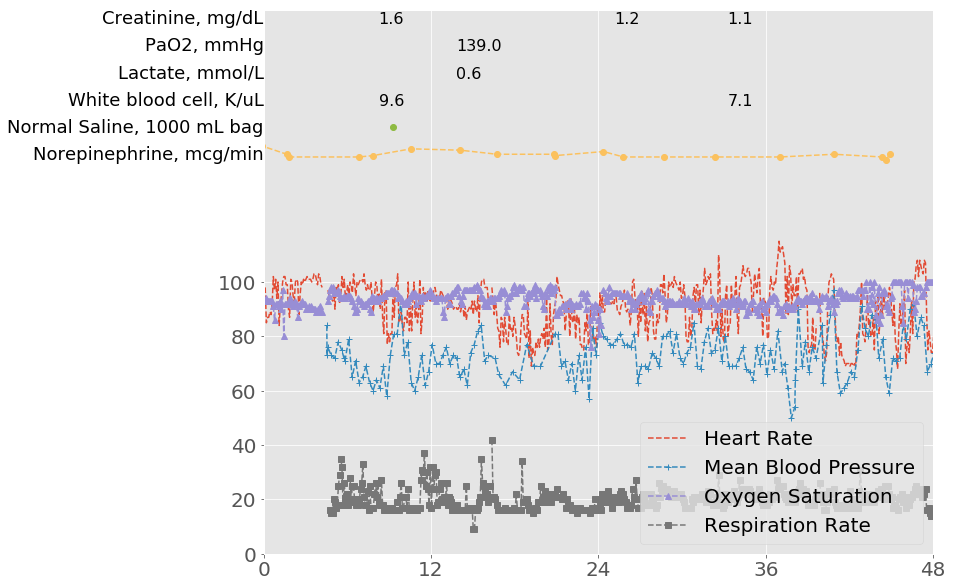
\includegraphics[width=1.0\textwidth]{img/ExamplePatient}
\caption{\emph{Visualization of a single patient's stay.} Data shown are a subset of all data available, and include: high granularity vital signs (dashed lines, sourced from \tblname{vitalPeriodic} and \tblname{vitalAperiodic}), nurse validated vital signs (solid markers, sourced from \tblname{nurseCharting}), blood product administration (green cross, sourced from \tblname{intakeOutput}), and laboratory measurements (sourced from \tblname{lab}). \label{fig:example_patient}}
\end{figure}

\section*{Author Contributions}\label{authorcontributions}
\addcontentsline{toc}{section}{Author Contributions}

AEWJ and TJP collaborated to publish the data and write the paper. JDR performed sample selection, provided the documentation for the process, and collaborated on the paper. LAC, RGM, and OB reviewed the paper and supervised the work.

\section*{Acknowledgements}\label{acknowledgments}
\addcontentsline{toc}{section}{Acknowledgments}

% --- REQUIREMENTS OF THIS SECTION --- %
% Text acknowledging non-author contributors. Acknowledgements should
% be brief, and should not include thanks to anonymous referees and
% editors, or effusive comments. Grant or contribution numbers may be
% acknowledged. Author contributions Please describe briefly the contributions
% of each author to this work on a separate line.
% ------------------------------------ %

The authors would like to thank the Philips eICU Research Institute and
Philips Healthcare for contribution of the data. The authors would also like to thank Andrew A. Kramer for insightful comments regarding the data, Dina Demner-Fushman for helpful feedback on the deidentification process, and Matthew M. McDermott for discussion around the manuscript.

\section*{Competing financial interests}\label{competing-interests}
\addcontentsline{toc}{section}{Competing interests}

The research and development was supported by grants NIH-R01-EB017205, NIH-R01-EB001659, and NIH-R01-GM104987 from the National Institutes of Health. The MIT Laboratory for Computational Physiology received funding from Philips Healthcare to undertake work on the database described in this paper. OB is an employee of Philips Healthcare.

\section*{Figure Legends}

% --- REQUIREMENTS OF THIS SECTION --- %
% Figure should be referred to using a consistent numbering scheme through
% the entire Data Descriptor. For initial submissions, authors may choose
% to supply this document as a single PDF with embedded figures, but
% separate figure image files must be provided for revisions and accepted
% manuscripts. In most cases, a Data Descriptor should not contain more
% than three figures, but more may be allowed when needed. We discourage
% the inclusion of figures in the Supplementary Information \textendash{}
% all key figures should be included here in the main Figure section.

% Figure legends begin with a brief title sentence for the whole figure
% and continue with a short description of what is shown in each panel,
% as well as explaining any symbols used. Legend must total no more
% than 350 words, and may contain literature references.
% ------------------------------------ %

\noindent
Figure \ref{fig:patient_organization}: Organization of patient tracking information. Each patient is identified by a unique integer: the \colname{uniquePid}. For each \colname{uniquePid}, a patient may have distinct hospitalizations denoted by \colname{patientHealthSystemStayId}. Finally, for each hospitalizations, a patient may have distinct unit stays, denoted by \colname{patientUnitStayId}. \colname{patientUnitStayId} is the identifier used for linking data across tables.\\

\noindent
Figure \ref{fig:example_patient}: Visualization of a single patient's stay. Data shown are a subset of all data available, and include: high granularity vital signs (dashed lines, sourced from \tblname{vitalPeriodic} and \tblname{vitalAperiodic}), nurse validated vital signs (solid markers, sourced from \tblname{nurseCharting}), blood product administration (green cross, sourced from \tblname{intakeOutput}), and laboratory measurements (sourced from \tblname{lab}).

\clearpage
\section*{Tables}

% Tables supporting the Data Descriptor. These can provide summary information
% (sample numbers, demographics, etc.), but they should generally not
% be used to present primary data (i.e. measurements). Tables containing
% primary data should be submitted to an appropriate data repository.

% Tables may be provided within the \LaTeX{} document or as separate
% files (tab-delimited text or Excel files). Legends, where needed,
% should be included here. Generally, a Data Descriptor should have
% fewer than ten Tables, but more may be allowed when needed. Tables
% may be of any size, but only Tables which fit onto a single printed
% page will be included in the PDF version of the article (up to a maximum
% of three).

% Table 1:
%	Demographics of the database

\begin{table}
\begin{tabular}{l|p{7cm}}
Data & Median [IQR], Mean (STD), or Number (\%) \\  \hline
Age, years (median [IQR]) & 65.00 [53.00,76.00] \\
Unit length of stay, days (median [IQR]) & 1.57
[0.82,2.97] \\
Hospital length of stay, days (median [IQR]) & 5.49
[2.90,10.04] \\
Admission height, cm (mean (std))* & 169.25 (13.69) \\
Admission weight, kg (mean (std))* & 83.93 (27.09) \\
Gender (n (\%)) & \\
\hspace{0.5cm} Male & 108,379 (53.96) \\
\hspace{0.5cm} Female & 92,303 (45.95) \\
\hspace{0.5cm} Other or Unknown & 177 (0.09) \\
Ethnicity (n (\%)) & \\
\hspace{0.5cm} African American & 21,308 (10.61) \\
\hspace{0.5cm} Asian & 3,270 (1.63) \\
\hspace{0.5cm} Caucasian & 155,285 (77.31) \\
\hspace{0.5cm} Hispanic & 7,464 (3.72) \\
\hspace{0.5cm} Native American & 1,700 (0.85) \\
\hspace{0.5cm} Other/Unknown & 11,832 (5.89) \\
Hospital discharge year (n (\%)) & \\
\hspace{0.5cm} 2014 & 95,513 (47.55) \\
\hspace{0.5cm} 2015 & 105,346 (52.45) \\
Unit type (n (\%)) & \\
\hspace{0.5cm} Coronary Care Unit/Cardiothoracic ICU & 15,290 (7.61) \\
\hspace{0.5cm} Cardiac Surgery ICU & 9,625 (4.79) \\
\hspace{0.5cm} Cardiothoracic ICU & 6,158 (3.07) \\
\hspace{0.5cm} Cardiac ICU & 12,467 (6.21) \\
\hspace{0.5cm} Medical ICU & 17,465 (8.70) \\
\hspace{0.5cm} Medical-Surgical ICU & 113,222 (56.37) \\
\hspace{0.5cm} Neurological ICU & 14,451 (7.19) \\
\hspace{0.5cm} Surgical ICU & 12,181 (6.06) \\
Status at unit discharge (n (\%)) & \\
\hspace{0.5cm} Alive & 189,918 (94.55) \\
\hspace{0.5cm} Expired & 10,907 (5.43) \\
\hspace{0.5cm} Unknown & 34 (0.02) \\
Status at hospital discharge (n (\%)) & \\
\hspace{0.5cm} Alive & 181,104 (90.16) \\
\hspace{0.5cm} Expired & 18,004 (8.96) \\
\hspace{0.5cm} Unknown & 1,751 (0.87) \\
\hline
\end{tabular}
\caption{Demographics of the 200,859 unit admissions in the database.
Note that multiple unit admissions can correspond to the same patient. *
Missing data excluded from calculation.
\label{tab:demographics}}
\end{table}

% Table 2:
%	APACHE Diagnosis frequency

\begin{center}
\begin{table}
\begin{tabular}{l|p{4cm}}
  APACHE Diagnosis & Number of patients(\%) \\\hline
Sepsis, pulmonary                                  &  6,823 (5.01) \\
Infarction, acute myocardial (MI)                  &  5,919 (4.34) \\
CVA, cerebrovascular accident/stroke               &  5,284 (3.88) \\
CHF, congestive heart failure                      &  4,840 (3.55) \\
Sepsis, renal/UTI (including bladder)              &  4,284 (3.14) \\
Diabetic ketoacidosis                              &  4,001 (2.94) \\
CABG alone, coronary artery bypass grafting        &  3,635 (2.67) \\
Rhythm disturbance (atrial, supraventricular)      &  3,474 (2.55) \\
Cardiac arrest (with or without respiratory arrest) &  3,377 (2.48) \\
Emphysema/bronchitis                               &  3,304 (2.43) \\
\hline
\end{tabular}
\caption{Most frequent admission diagnoses as coded using the APACHE IV
diagnosis system. Percentages are calculated for the subset of 136,236 unit
stays with an APACHE IV hospital mortality prediction. UTI is urinary tract infection.
\label{tab:apachedx}}
\end{table}
\end{center}

% Table 3:
%	APACHE Diagnosis frequency

\begin{center}
\begin{table}
\begin{tabular}{l|p{4cm}}
APACHE Diagnosis category & Number of patients (\%) \\ \hline
Sepsis                                   & 18,087 (16.40) \\
Cerebrovascular accident                 &  9,758 (8.85) \\
Cardiac Arrest                           &  9,135 (8.28) \\
Acute Coronary Syndrome                  &  8,343 (7.57) \\
Respiratory medicine                     &  7,970 (7.23) \\
Gastrointestinal Bleed                   &  7,277 (6.60) \\
Congestive Heart Failure                 &  5,884 (5.34) \\
Trauma                                   &  5,592 (5.07) \\
Coronary Artery Bypass Graft             &  4,771 (4.33) \\
Neurological                             &  4,640 (4.21) \\
Pneumonia                                &  4,577 (4.15) \\
Diabetic Ketoacidosis                    &  4,384 (3.98) \\
Overdose                                 &  4,268 (3.87) \\
Asthma/Emphysema                         &  3,948 (3.58) \\
Other cardiovascular disease             &  3,593 (3.26) \\
Valvular disorders                       &  2,795 (2.53) \\
Coma                                     &  2,082 (1.89) \\
Acute renal failure                      &  1,932 (1.75) \\
Gastrointestinal obstruction             &  1,232 (1.12) \\
\hline
\end{tabular}
\caption{Most frequent categories of APACHE diagnosis using clinically
meaningful groups defined in the code repository~\cite{eicu-code}.
Patients who are missing APACHE IV hospital mortality
predictions are excluded (N=64,623, includes burns patients, in-hospital
readmissions, short length of stay, and other APACHE exclusion criteria).
\label{tab:apachedx_groups}}
\end{table}
\end{center}

% Table 4:
%	List of tables

\begin{center}
\begin{table}
\begin{tabular}{p{4.4cm}|p{10.5cm}}
Table name & Type of data  \\\hline
  \tblname{admissionDrug} & \textbf{Care documentation}: Medications taken prior to unit admission.  \\
  \tblname{admissionDx} & \textbf{APACHE}: Admission diagnoses and other APACHE information.  \\
  \tblname{allergy} & \textbf{Care documentation}: Known patient allergies.  \\
  \tblname{apacheApsVar} & \textbf{APACHE}: Physiology score components used in predictions.  \\
  \tblname{apachePredVar} & \textbf{APACHE}: Other components used in predictions.  \\
  \tblname{apachePatientResult} & \textbf{APACHE}: Predictions made by APACHE IV and IVa.  \\
  \tblname{carePlanCareProvider} & \textbf{Care plan}: Details regarding managing or consulting providers. \\
  \tblname{carePlanEOL} & \textbf{Care plan}: End of life care planning. \\
  \tblname{carePlanGeneral} & \textbf{Care plan}: Plans for patient care, often including end of life care. \\
  \tblname{carePlanGoal} & \textbf{Care plan}: Stated goals of care for the patient.  \\
  \tblname{carePlanInfectiousDisease} & \textbf{Care plan}: Precautions for patient related to infectious disease.  \\
  \tblname{customLab}   &  \textbf{Care documentation}: Infrequent, unstandardized laboratory tests. \\
  \tblname{diagnosis} &  \textbf{Care documentation}: Structured record of active problems. \\
  \tblname{hospital}  & \textbf{Administration}: Hospital level survey information: bed size, teaching status, and US region.  \\
  \tblname{infusionDrug} &  \textbf{Care documentation}: Continuous infusions administered.  \\
  \tblname{intakeOutput} &  \textbf{Care documentation}: Intake and output recorded for patients. \\
  \tblname{lab} &  \textbf{Care documentation}: Laboratory measurements for patient derived specimens. \\
  \tblname{medication} &  \textbf{Care documentation}: Prescribed medications usually interfaced from a local pharmacy system. \\
  \tblname{microLab}   &  \textbf{Care documentation}: Manually entered microbiology information. \\
  \tblname{note}   &  \textbf{Care documentation}: Semi-structured notes entered by the physician or physician extender responsible. \\
  \tblname{nurseAssessment}   &  \textbf{Care documentation}: Documentation for patient items such as pain, psychosocial status, etc. \\
  \tblname{nurseCare}   &  \textbf{Care documentation}: Documentation for patient items such as nutrition, wound care, drain/tube care, restraints, etc. \\
  \tblname{nurseCharting} &  \textbf{Care documentation}: Primary location for information charted at the bed side such as vital signs. \\
  \tblname{pastHistory} &  \textbf{Care documentation}: Structured list detailing patient's health status prior to presentation in the unit.  \\
  \tblname{patient}  &  \textbf{Administration}: Demographic and administrative information regarding the patient and their unit/hospital stay.  \\
  \tblname{physicalExam}   &  \textbf{Care documentation}: Semi-structured results of physical examinations performed. \\
  \tblname{respiratoryCare}   &  \textbf{Care documentation}: Documentation for airway structure, cuff pressures, and other respiratory related details. \\
  \tblname{respiratoryCharting}   &  \textbf{Care documentation}: Primary location for ventilator setting information including tidal volumes, pressure settings, etc. \\
  \tblname{treatment} & \textbf{Care documentation}: Structured list detailing active treatments provided to the patient  \\
  \tblname{vitalAperiodic} & \textbf{Monitor data}: Unevenly sampled vital sign measurements such as non-invasive blood pressure.  \\
  \tblname{vitalPeriodic} & \textbf{Monitor data}: Five minute medians for continuous vital sign measurements such as invasive blood pressure.  \\
 \hline
 \end{tabular}
 \caption{List of tables available in the eICU Collaborative Research Database (v2.0). Short descriptions of data contained in the table are provided. APACHE: Acute Physiology, Age, and Chronic Health Evaluation.
 \label{tab:tables_available}}
\end{table}
\end{center}

% Table 5:
%	Hospital level information

\begin{center}
\begin{table}
\begin{tabular}{l|p{4cm}|p{4cm}}
Hospital level factor & Number of hospitals (\%) & Number of patients (\%) \\ \hline
Bed capacity & & \\
\hspace{0.5cm} \textless{}100 & 46 (22.12\%) & 12,593 (6.27\%) \\
\hspace{0.5cm} 100 - 249 & 62 (29.81\%) & 41,966 (20.89\%) \\
\hspace{0.5cm} 250 - 499 & 35 (16.83\%) & 45,716 (22.76\%) \\
\hspace{0.5cm} \textgreater{}= 500 & 23 (11.06\%) & 75,305 (37.49\%) \\
\hspace{0.5cm} Unknown & 42 (20.19\%) & 25,279 (12.59\%) \\
Teaching status & & \\
\hspace{0.5cm} False & 189 (90.87\%) & 149,181 (74.27\%) \\
\hspace{0.5cm} True & 19 (9.13\%) & 51,678 (25.73\%) \\
Region & & \\
\hspace{0.5cm} Midwest & 70 (33.65\%) & 65,950 (32.83\%) \\
\hspace{0.5cm} Northeast & 13 (6.25\%) & 14,429 (7.18\%) \\
\hspace{0.5cm} South & 56 (26.92\%) & 60,294 (30.02\%) \\
\hspace{0.5cm} West & 43 (20.67\%) & 46,348 (23.07\%) \\
\hspace{0.5cm} Unknown & 26 (12.50\%) & 13,838 (6.89\%) \\
\hline
\end{tabular}
\caption{Hospital level information. Information includes the region of the US the hospital is located in, whether it is a teaching hospital, the bed capacity, and the number of patients with data available for these hospital subtypes.
\label{tab:hospital_info}}
\end{table}
\end{center}

% Table 6:
%	Organ system for problems

\begin{center}
\begin{table}
\begin{tabular}{l|p{4cm}}
Diagnosis group & Number of patients (\%) \\\hline
Cardiovascular                           & 104,264 (11.15\%) \\
Pulmonary                                & 64,222 (8.15\%) \\
Neurologic                               & 51,609 (7.28\%) \\
Renal                                    & 43,009 (6.38\%) \\
Endocrine                                & 35,519 (6.15\%) \\
Gastrointestinal                         & 35,223 (6.10\%) \\
Infectious diseases                      & 20,316 (6.01\%) \\
Hematology                               & 19,611 (5.32\%) \\
Burns/trauma                             & 9,208 (5.13\%) \\
Oncology                                 & 7,954 (4.72\%) \\
Toxicology                               & 7,185 (4.47\%) \\
Surgery                                  & 5,723 (3.97\%) \\
General                                  & 1,698 (3.91\%) \\
Transplant                               &   770 (3.75\%) \\
Obstetrics/gynecology                    &    46 (3.52\%) \\
Genitourinary                            &    26 (3.18\%) \\
Musculoskeletal                          &    19 (2.98\%) \\
\hline
\end{tabular}
\caption{Organ system for problems documented during patient unit stays. More than one problem can be documented for a single patient, and therefore the percentages will add up to greater than 100\%.
\label{tab:organ_system}}
\end{table}
\end{center}

% Table 7:
%	vitalperiodic data

\begin{landscape}
\begin{table}
\begin{tabular}{l|p{3.2cm}|p{3.7cm}|p{4.7cm}}
  Data type  &  Column name  &  Number of patients (\%)  &
  Total number of observations (average patient-wise)  \\ \hline
  Heart rate                               & \colname{heartrate}          & 192277 (95.73\%) & 145,979,794 (759.2) \\
  Peripheral oxygen saturation             & \colname{sao2}               & 189646 (94.42\%) & 132,908,266 (700.8) \\
  Respiration rate                         & \colname{respiration}        & 178051 (88.64\%) & 128,501,032 (721.7) \\
  ST level                                 & \colname{st2}                &  98886 (49.23\%) & 59,949,273 (606.2) \\
  ST level                                 & \colname{st1}                &  95643 (47.62\%) & 56,604,917 (591.8) \\
  ST level                                 & \colname{st3}                &  92752 (46.18\%) & 55,201,239 (595.1) \\
  Invasive mean blood pressure             & \colname{systemicmean}       &  46975 (23.39\%) & 28,060,870 (597.4) \\
  Invasive systolic blood pressure         & \colname{systemicsystolic}   &  46667 (23.23\%) & 27,834,959 (596.5) \\
  Invasive diastolic blood pressure        & \colname{systemicdiastolic}  &  46661 (23.23\%) & 27,833,847 (596.5) \\
  Central venous pressure                  & \colname{cvp}                &  28698 (14.29\%) & 19,157,758 (667.6) \\
  Temperature                              & \colname{temperature}        &  19419 (9.67\%) & 13,203,289 (679.9) \\
  Mean pulmonary artery pressure           & \colname{pamean}             &  10893 (5.42\%) & 4,150,132 (381.0) \\
  Diastolic pulmonary artery pressure      & \colname{padiastolic}        &  10792 (5.37\%) & 4,120,636 (381.8) \\
  Systolic pulmonary artery pressure       & \colname{pasystolic}         &  10789 (5.37\%) & 4,121,138 (382.0) \\
  End tidal carbon dioxide concentration   & \colname{etco2}              &   8346 (4.16\%) & 4,423,333 (530.0) \\
  Intracranial pressure                    & \colname{icp}                &   1634 (0.81\%) & 2,631,227 (1610.3) \\
  \hline
  \end{tabular}
 \caption{Data available in \tblname{vitalPeriodic} table, including the
number of patients who have at least one measurement, the total number
of observations available, and the average number of observations
available per patient for patients who have at least one measurement recorded.
\label{tab:vitalperiodic}}
 \end{table}
\end{landscape}

% Table 8:
%	Data completion grouped by table

\begin{table}
\begin{tabular}{l|p{1.25cm}|p{1.0cm}|p{1.25cm}|p{1.25cm}|p{1.25cm}}
& \multicolumn{5}{c}{Coverage} \\ \hline
Table Name &
None &
Low & % coverage (0-20\%)
Medium & % coverage (20-60\%)
High & % coverage (60-80\%)
Excellent \\ % coverage (80-100\%)
\hline
\tblname{admissionDx}                    &  0.48 &  0.48 &  5.77 & 15.38 & 77.88 \\
\tblname{admissionDrug}                  & 41.35 & 24.52 & 19.23 &  2.88 & 12.02 \\
\tblname{allergy}                        & 10.58 & 20.67 & 63.46 &  5.29 &  0.00 \\
\tblname{apacheApsVar}                   &  0.00 &  0.48 &  6.73 & 14.90 & 77.88 \\
\tblname{apachePredVar}                  &  0.00 &  0.48 &  6.73 & 14.90 & 77.88 \\
\tblname{apachePatientResult}            &  8.65 &  0.96 & 16.83 & 12.98 & 60.58 \\
\tblname{carePlanCareProvider}           &  0.96 &  0.96 & 12.02 & 12.98 & 73.08 \\
\tblname{carePlanEOL}                    & 53.85 & 46.15 &  0.00 &  0.00 &  0.00 \\
\tblname{carePlanGeneral}                &  0.48 &  0.00 &  0.48 &  2.40 & 96.63 \\
\tblname{carePlanGoal}                   & 62.98 & 27.40 &  0.96 &  4.33 &  4.33 \\
\tblname{carePlanInfectiousDisease}      & 53.85 & 38.94 &  6.73 &  0.48 &  0.00 \\
\tblname{customLab}                      & 92.79 &  4.81 &  0.48 &  0.48 &  1.44 \\
\tblname{diagnosis}                      &  0.48 &  0.48 & 11.54 & 11.54 & 75.96 \\
\tblname{infusionDrug}                   & 26.92 & 16.35 & 40.38 &  9.62 &  6.73 \\
\tblname{intakeOutput}                   &  2.40 &  3.85 &  5.29 & 12.02 & 76.44 \\
\tblname{lab}                            &  0.48 &  0.00 &  0.48 &  2.88 & 96.15 \\
\tblname{medication}                     & 16.35 &  7.21 &  2.40 &  1.92 & 72.12 \\
\tblname{microLab}                       & 89.42 &  5.77 &  3.85 &  0.96 &  0.00 \\
\tblname{note}                           &  0.00 &  0.00 &  3.37 & 16.83 & 79.81 \\
\tblname{nurseAssessment}                & 92.31 &  1.92 &  0.96 &  0.00 &  4.81 \\
\tblname{nurseCare}                      & 93.27 &  0.96 &  0.96 &  0.00 &  4.81 \\
\tblname{nurseCharting}                  &  0.48 &  0.96 &  1.92 &  4.33 & 92.31 \\
\tblname{pastHistory}                    &  0.48 &  0.48 &  4.33 & 17.31 & 77.40 \\
\tblname{physicalExam}                   &  0.48 &  0.48 &  3.85 & 17.79 & 77.40 \\
\tblname{respiratoryCare}                & 24.52 & 41.35 & 33.17 &  0.48 &  0.48 \\
\tblname{respiratoryCharting}            & 11.06 & 15.38 & 35.58 &  9.62 & 28.37 \\
\tblname{treatment}                      &  6.25 &  3.37 & 12.98 & 11.54 & 65.87 \\
\tblname{vitalAperiodic}                 &  0.96 &  0.00 &  3.85 &  5.29 & 89.90 \\
\tblname{vitalPeriodic}                  &  0.96 &  0.00 &  3.37 &  2.40 & 93.27 \\
\hline
\end{tabular}
\caption{Data completion grouped by table and tabulated by hospitals.
Data completion is assessed by the percent of patient unit stays with
data. For example, if between 20-60\% of \colname{patientUnitStayId} at a
hospital have data, then we term this medium coverage, and 5.77\% of
hospitals have medium coverage for \tblname{admissionDx}.
Coverage groups are: none (0\%), low (0-20\%), medium (20-60\%), high (60-80\%), and excellent (80-100\%).
Note that this table does not necessarily represent reliability of data collection
as the expected prevalence of documentation for each table varies.
\label{tab:data_completion}}
\end{table}

% Table 9:
%	XXX

\clearpage
\begin{thebibliography}{1}
\expandafter\ifx\csname url\endcsname\relax
  \def\url#1{\texttt{#1}}\fi
\expandafter\ifx\csname urlprefix\endcsname\relax\def\urlprefix{URL }\fi
\providecommand{\bibinfo}[2]{#2}
\providecommand{\eprint}[2][]{\url{#2}}

\bibitem{kelly2014intensive}
Kelly F.E., Fong K., Hirsch N., and Nolan J.P.
\newblock Intensive care medicine is 60 years old: the history and future of
  the intensive care unit.
\newblock {\em Clinical medicine}, 14(4):376--379 (2014).

\bibitem{adhikari2010critical}
Adhikari N.K., Fowler R.A., Bhagwanjee S., and Rubenfeld G.D.
\newblock Critical care and the global burden of critical illness in adults.
\newblock {\em The Lancet}, 376(9749):1339--1346 (2010).

\bibitem{Celi2013loop}
Celi L.A., Mark R.G., Stone D.J., and Montgomery R.A.
\newblock {``Big Data'' in the Intensive Care Unit: Closing the Data Loop}.
\newblock {\em Am J Respir Crit Care Med}, 187(11):1157--1160 (2013).

\bibitem{johnson2016machine}
Johnson A.E.W., Ghassemi M., Nemati S., Niehaus K.E., Clifton D.A., and Clifford G.D.
\newblock Machine learning and decision support in critical care.
\newblock {\em Proceedings of the IEEE}, 104(2):444--466 (2016).

\bibitem{lilly2014multicenter}
Lilly C.M., McLaughlin J.M., Zhao H., Baker S.P., Cody S.,
  and Irwin R.S.
\newblock A multicenter study of icu telemedicine reengineering of adult
  critical care.
\newblock {\em CHEST Journal}, 145(3):500--507 (2014).

\bibitem{mcshea2010eicu}
McShea M., Holl R., Badawi O., Riker R.R., and Silfen E.
\newblock The {eICU} research institute-a collaboration between industry, health-care providers, and academia.
\newblock {\em IEEE Engineering in Medicine and Biology Magazine}, 29(2):18--25 (2010).

\bibitem{MIMIC2011}
Saeed M., Villarroel M., Reisner A.T., Clifford G., Lehman L.W., Moody G., Heldt T., Kyaw T.H., Moody B., and Mark R.G.
\newblock Multiparameter Intelligent Monitoring in Intensive Care {II} ({MIMIC-II}): a public-access intensive care unit database. \newblock {\em Critical care medicine}, 39(5):952-960 (2011).

\bibitem{MIMIC2016}
Johnson A.E.W., Pollard T.J., Shen L., Lehman L.H., Feng M., Ghassemi M., Moody B., Szolovits P., Celi L.A., and Mark R.G.
\newblock {MIMIC-III}, a freely accessible critical care database.
\newblock {\em Scientific Data}, 3 (2016).

\bibitem{HIPAA}
United States. Cong. House.
\newblock Health Insurance Portability and Accountability Act of 1996.
\newblock \emph{104th Congress}, https://www.gpo.gov/fdsys/pkg/PLAW-104publ191/html/PLAW-104publ191.htm (\bibinfo{year}{(1996)}).

\bibitem{neamatullah2008automated}
Neamatullah I., Douglass M. M., Lehman L. H., Reisner A., Villarroel M., Long W. J., Szolovits P., Moody G. B., Mark R. G. and Clifford G. D.
\newblock Automated de-identification of free-text medical records.
\newblock {\em BMC medical informatics and decision making}, 8(1):1--32 (2008).

\bibitem{finney2011efficient}
Finney J.M., Walker A.S., Peto T.M., and Wyllie D.H.
\newblock An efficient record linkage scheme using graphical analysis for
  identifier error detection.
\newblock {\em BMC Medical Informatics and Decision Making}, 11(1):7 (\bibinfo{year}{2011}).

\bibitem{eicu-data-paper}
Johnson A. E. W. and Pollard T. J.
\newblock MIT-LCP/eicu-data-paper: eICU-CRD Code for Data Descriptor.
\newblock \emph{Zenodo}, https://doi.org/10.5281/zenodo.1248994 (\bibinfo{year}{2018}).

\bibitem{eicu-code}
Pollard T. J., Johnson A. E. W., Badawi O., Naumann T. J., Rincon T., and Raffa J. D.
\newblock MIT-LCP/eicu-code: eICU-CRD Code Repository.
\newblock \emph{Zenodo}, https://doi.org/10.5281/zenodo.1249016 (\bibinfo{year}{2018}).

\bibitem{tableone}
Pollard T. J., Johnson A. E. W., Raffa J, and Mark R. G.
\newblock tableone: An open source Python package for producing summary statistics for research papers.
\newblock {\em JAMIA Open}. https://doi.org/10.1093/jamiaopen/ooy012 (\bibinfo{year}{2018}).

\bibitem{zimmerman2006acute}
Zimmerman J.E., Kramer A.A., McNair D.S., and Malila F.M.
\newblock Acute physiology and chronic health evaluation ({APACHE}) {IV}: hospital
  mortality assessment for today’s critically ill patients.
\newblock {\em Critical Care Medicine}, 34(5):1297--1310 (2006).

\bibitem{physionet-ref}
\bibinfo{author}{Goldberger, A.L.}, \bibinfo{author}{Amaral, L.A.N.},
\bibinfo{author}{Glass, L.}, \bibinfo{author}{Hausdorff, J.M.},
\bibinfo{author}{Ivanov, P.Ch.}, \bibinfo{author}{Mark, R.G.},
\bibinfo{author}{Mietus, J.E.}, \bibinfo{author}{Moody, G.B.},
\bibinfo{author}{Peng, C.-K.} \& \bibinfo{author}{Stanley, H.E.},
\newblock \bibinfo{title}{{PhysioBank, PhysioToolkit, and PhysioNet.}}
\newblock \emph{\bibinfo{journal}{Circulation}}
  \textbf{\bibinfo{volume}{101}}, \bibinfo{pages}{e215----e220}
  (\bibinfo{year}{2000}).

\bibitem{eicu-website}
Johnson A. E. W., Pollard T. J., Badawi O.
\newblock \bibinfo{title}{{eICU Collaborative Research Database: Documentation and Website.}}
\newblock https://eicu-crd.mit.edu
(\bibinfo{year}{2018}).

\bibitem{citicourse}
Braunschweiger, P. and Goodman, K. W.
\newblock The CITI program: an international online resource for education in human subjects protection and the responsible conduct of research
\newblock {\em Academic Medicine}, 82(9):861--864 (\bibinfo{year}{2007}).
%\newblock \bibinfo{title}{{Collaborative Institutional~Training Initiative Human subjects research, 2017.}}
%\newblock \emph{\bibinfo{journal}{https://about.citiprogram.org/en/homepage/}}

\bibitem{Wilson2014}
Wilson G., Aruliah D.A., Brown C.T., Chue Hong N.P., Davis M., Guy R.T., Haddock S.H., Huff K., Mitchell I.M., Plumbley M.D., Waugh B., White E.P., and Wilson P.
\newblock {Best practices for scientific computing.}
\newblock {\em PLOS Biology}, 12(1):e1001745 (2014).

\bibitem{johnson2017reproducibility}
Johnson A. E. W., Pollard T. J., and Mark R. G.
\newblock Reproducibility in critical care: a mortality prediction case study.
\newblock {\em Proceedings of Machine Learning Research}, 68:361--376 (2017).

\bibitem{pergra2007ipython}
P\'erez F. and Granger B.
\newblock {IP}ython: a system for interactive scientific computing.
\newblock {\em Computing in Science and Engineering}, 9(3):21--29 (2007).

\bibitem{kluyver2016jupyter}
Kluyver T., Ragan-Kelley B., P{\'e}rez F., Granger B.E., Bussonnier M., Frederic J., Kelley K., Hamrick J.B., Grout J., Corlay S., et al.
\newblock Jupyter notebooks-a publishing format for reproducible computational
  workflows.
\newblock In {\em ELPUB}, pages 87--90 (2016).

\end{thebibliography}

\section*{Data Citations}

1. Pollard, T.J., Johnson, A.E.W., Raffa, J., Badawi, O. \emph{The eICU Collaborative Research Database}. https://dx.doi.org/10.13026/C2WM1R (2018).

\end{document}
